\begin{ledgroupsized}[r]{120mm}
\footnotesize
\pstart
\noindent\textbf{Überlieferung:}
\pend
\end{ledgroupsized}
\begin{ledgroupsized}[r]{114mm}
\footnotesize
\pstart \parindent -6mm
\makebox[6mm][l]{\textit{L}}%
Konzept:
LH~XXXVII~5~Bl.~42. 
Ein Blatt (16,5 x 13,5 cm);
oberer, unterer und linker Rand beschnitten, rechter Rand ausgefranst;
Papiererhaltungsmaßnahmen.
\href{\Scan{LH_37_05_042wz}}%
{Gegenmarke}
eines Wasserzeichens.
Zweidrittel Seiten auf Bl.~42~r\textsuperscript{o}; Rückseite leer.
\pend
\end{ledgroupsized}
\vspace{5mm}
\begin{ledgroup}
\footnotesize
\pstart
\noindent%
\textbf{Datierungsgründe:}
Das Wasserzeichen ist für den Zeitraum Oktober 1690 
bis November 1694 mehrfach belegt.
\pend 
\end{ledgroup}
\selectlanguage{latin}
\vspace{8mm}
\pstart%
\normalsize%
\noindent%
\href{\Scan{LH_37_05_042r}}%
{\lbrack42~r\textsuperscript{o}\rbrack}
\pend %
\nobreak\begin{edfigure}[0.5em]%
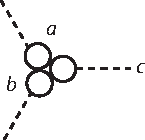
\includegraphics[scale=1]{gesamttex/edit_VIII-4/images/LH_37_05_042_d1.pdf} 
\edcaption[0.25em]{\lbrack\textit{Fig.~1}\rbrack}
\end{edfigure}
\pstart
\noindent
Concurrunt
\edtext{tres globi}{\lemma{tres}\Bfootnote{%
\textit{(1)}~Circuli %
\textit{(2)}~globi~\textit{L}}} 
aequales\indexS{globi tres aequales concurrentes} 
\edtext{aequali celeritate triangulatim}{\lemma{}\Bfootnote{aequali celeritate triangulatim \textit{erg.~L}}}.
Centrum grav.\indexS{centrum gravitatis}\ eorum quiescit ante ictum,%
\indexS{ictus} quiescet ergo et  
\edtext{post ictum.\indexS{ictus} Nullus}{\lemma{post ictum.}\Bfootnote{%
\textit{(1)}~Et cum %
\textit{(2)}~Necesse est %
\textit{(3)}~Nullus~\textit{L}}}
globus\indexS{globus} progredi potest, nam alioqui progrederentur omnes, quod impossibile. Si unus quiesceret, omnes quiescent, ergo periisset 
\edtext{vis.\indexS{vis} Reflecterentur}{\lemma{vis.}\Bfootnote{%
\textit{(1)}~Idem est si unius mot %
\textit{(2)}~Reflecterentur~\textit{L}}} 
ergo, et quidem qua venerunt 
\edtext{celeritate, nam}{\lemma{celeritate,}\Bfootnote{%
\textit{(1)}~alioqui %
\textit{(2)}~nam~\textit{L}}} 
si vel unus tardius iret, omnes tardius irent, et vis\indexS{vis} perisset. 
\pend
\pstart
Ponamus unum \textit{c} celerius ferri, sed duos \textit{a} et \textit{b}
eandem habere velocitatem. Fingatur Tabula\indexS{tabula} moveri 
celeritate centri gravitatis,\indexS{celeritas centri gravitatis}\indexS{centrum gravitatis} 
sed \textit{a}, \textit{b}, \textit{c}, 
in Tabula\indexS{tabula} aeque 
\edtext{celeriter, et}{\lemma{celeriter,}\Bfootnote{%
\textit{(1)}~et fiet %
\textit{(2)}~et~\textit{L}}} 
habebimus quid fiat, 
nempe motui tabulae\indexS{motus tabulae} %
\edtext{addit\lbrack a\rbrack}{%
\lemma{}%
\Bfootnote{%
additus %
\textit{L ändert Hrsg.}}}
cujusque reflexio\indexS{reflexio} 
aequalis et contraria adventuum\indexS{adventus}
in tabula\indexS{tabula}, dat motum absolutum\indexS{motus absolutus}. 
Sed si cuilibet ex globis\indexS{globus} propria sit velocitas, an duplicem tabulam\indexS{tabula} 
fingemus? Seu navim in navi?\indexS{navis in navi} 
\pend
\pstart
Sed hoc puto perplexum. Fingamus duos globos\indexS{globus} ferri in eadem navi,\indexS{navis} sic ut navis feratur eorum 
\indexS{centrum commune speciale}centro communi speciali\lbrack,\rbrack\ 
\edtext{motus his duobus attributi.}{\lemma{}\Bfootnote{motus his duobus  attributi \textit{erg.~L}}}
Haec navis feratur in alia navi;\indexS{navis in navi} quae moveatur motu centri grav.\ com.\indexS{motus centri gravitatis communis}\indexS{centrum gravitatis commune}\ et simul in ea feratur tertius globus,\indexS{globus} qui occurrat duobus prioribus 
in sua navi\indexS{navis} latis. Sed ista puto perplexiora.
\pend 
\begin{edfigure}%
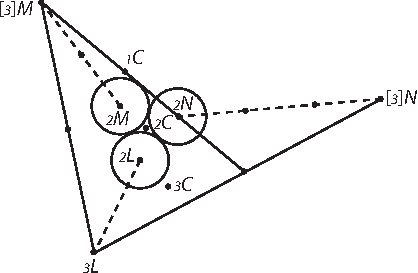
\includegraphics[scale=1]{gesamttex/edit_VIII-4/images/LH_37_05_042_d2.pdf}
\edcaption[0pt]{%
\edtext{\lbrack\textit{Fig.~2}\rbrack}{%
\lemma{\lbrack\textit{Fig.~2}\rbrack}%
\Cfootnote[nonum]{%
Ein gestrichener Entwurf zum Diagramm wird nicht wiedergegeben. Die Bezeichnungen der Punkte \textit{\ind{3}M} und \textit{\ind{3}N} (bei Leibniz \textit{\ind{2}M} und \textit{\ind{2}N}) ändert Hrsg.}}}
\end{edfigure}
\pstart
Vera methodus\indexS{methodus per virium respectivarum combinationem} mea est, per virium respectivarum\indexS{vis respectiva} combinationem\indexS{combinatio virium respectivarum} utcunque.
Globus\indexS{globus in globum oblique incurrens} \textit{L} incurrit in globum \textit{N} 
\edtext{oblique, et hinc}{\lemma{oblique}\Bfootnote{%
\textit{(1)}~, ictu cujus vis %
\textit{(2)}~, et hinc~\textit{L}}} 
patet vis respectiva inter ipsos particularis.\indexS{vis respectiva particularis} Sed similiter globus\indexS{globus} \textit{M} in globum \textit{N}. 
Vis respectiva totalis\indexS{vis respectiva totalis} esset intensio\indexS{intensio funis} trium funium\indexS{funis} tres globos 
connectentium per discessum. Et ita notandum si plures sint globi,\indexS{globus} 
quemlibet cuilibet connexum intelligi. 
NB Si sint 
\edtext{tres vis}{\lemma{tres}\Bfootnote{%
\textit{(1)}~\bars{concipi \textit{streicht Hrsg.}} possunt %
\textit{(2)}~vis~\textit{L}}} 
respectiva\indexS{vis respectiva} componi potest concipiendo tum qua celeritate centrum grav.\ 
\edtext{commune\indexS{centrum gravitatis commune} \textit{L}}{%
\lemma{commune}%
\Bfootnote{%
\textit{(1)}~\textit{M} et %
\textit{(2)}~\textit{L} %
\textit{L}%
}}
et \textit{M} recedit ab \textit{N}, 
tum qua \textit{M} et \textit{L} recedunt a se invicem.
Eadem quantitas alia hypothesi prodire debet.
\pend 
